\documentclass[a4paper]{article}

%% Language and font encodings
% \usepackage{fontspec}
\usepackage{listings}
\usepackage{enumitem}
\usepackage{float}

%% Sets page size and margins
\usepackage[a4paper,top=3cm,bottom=2cm,left=3cm,right=3cm,marginparwidth=1.75cm]{geometry}

\usepackage{graphicx}
% \usepackage{booktabs}

% UNCOMMENT FOR WATERMARK
% \usepackage{draftwatermark}
% \SetWatermarkText{Working Draft}
% \SetWatermarkScale{1}

%% Useful packages
\usepackage{amsmath,amsthm,amssymb,amsfonts}
\usepackage{graphicx}
\usepackage{xcolor}
\usepackage[colorinlistoftodos]{todonotes}
\usepackage[colorlinks=true, allcolors=blue]{hyperref}
\usepackage{ragged2e}

\newcommand{\R}{\mathbb{R}}
\newcommand{\N}{\mathbb{N}}
\newcommand{\Z}{\mathbb{Z}}
\providecommand{\C}{\mathbb{C}}
\newcommand{\classname}[1]{\texttt{#1}}


\theoremstyle{definition}
\newtheorem{defin}{Definição}

\theoremstyle{plain}
\newtheorem{theorem}[defin]{Teorema}
\newtheorem{corollary}[defin]{Corolário}

\usepackage{caption}

%\setcounter{section}{-1}
\usepackage{subfig}
%\setlength\parindent{0pt}


\title{HW 6: Probabilistic Reasoning\\ (Programming Assignment)}

\author{CMSC 421 Spring 2022\\
\textbf{Due date: 11:59 PM, May 9, 2022}}

\date{}
\begin{document}
\maketitle

\section*{Introduction}

\subsection*{Goal}

In this programming assignment, you will localize a car in a racetrack, and analyze a competitive situation on the racetrack and its effects on successfully overtaking an opponent, avoiding collision, and winning a race. In order to localize the car, you will create a particle filter (and a Kalman filter for extra credit), and in order to analyze situations, you will implement a Bayesian network to model conditional dependencies between situations and outcomes. We will then ask you some questions about your implementations and performance.

\subsection*{Setup}

\begin{enumerate}
    \item Clone the repo at \url{https://github.com/jdkanu/cmsc421-p3}
    \item Run \texttt{pip3 install -r requirements.txt} to install dependencies
    %TODO \item install requirements - If you're doing the kalman filter, install filterpy.
    \item Try running \texttt{python3 gui.py} and driving around the track with your arrow keys. You should see a blue car at the bottom, and it should move according to your keyboard inputs.
\end{enumerate}

\subsection*{Directory structure}

\begin{tabbing}
    Files you will edit:\\
    \texttt{particle\_filter.py} \hspace{2em} \= Write your particle filter code in here \\
    \texttt{bayesian\_network.py} \> Write your bayesian network code in here\\
    \texttt{kalman\_filter.py} \> Write your kalman filter code in here\\\\
    
    Files you may edit, though it is not required:\\
    \texttt{plots.py} \> Generates plots for particle filtering and Kalman filtering\\\\
    
    Files you will not edit:\\
    \texttt{data} \> Directory containing various data objects to define simulator \\
    \texttt{gui.py} \> GUI for interacting with simulator\\
    \texttt{car.py} \> Car in simulator\\
    \texttt{probability.py} \> Some code from AIMA code repo providing Bayesian network\\
    \texttt{racetrack.py} \> Racetrack in simulator\\
    \texttt{simulator.py} \> Simulator representing world with car and racetrack\\
    \texttt{utils.py} \> Utility functions
\end{tabbing}

\begin{figure}[t!]%
    \centering
    \subfloat[\centering ]{{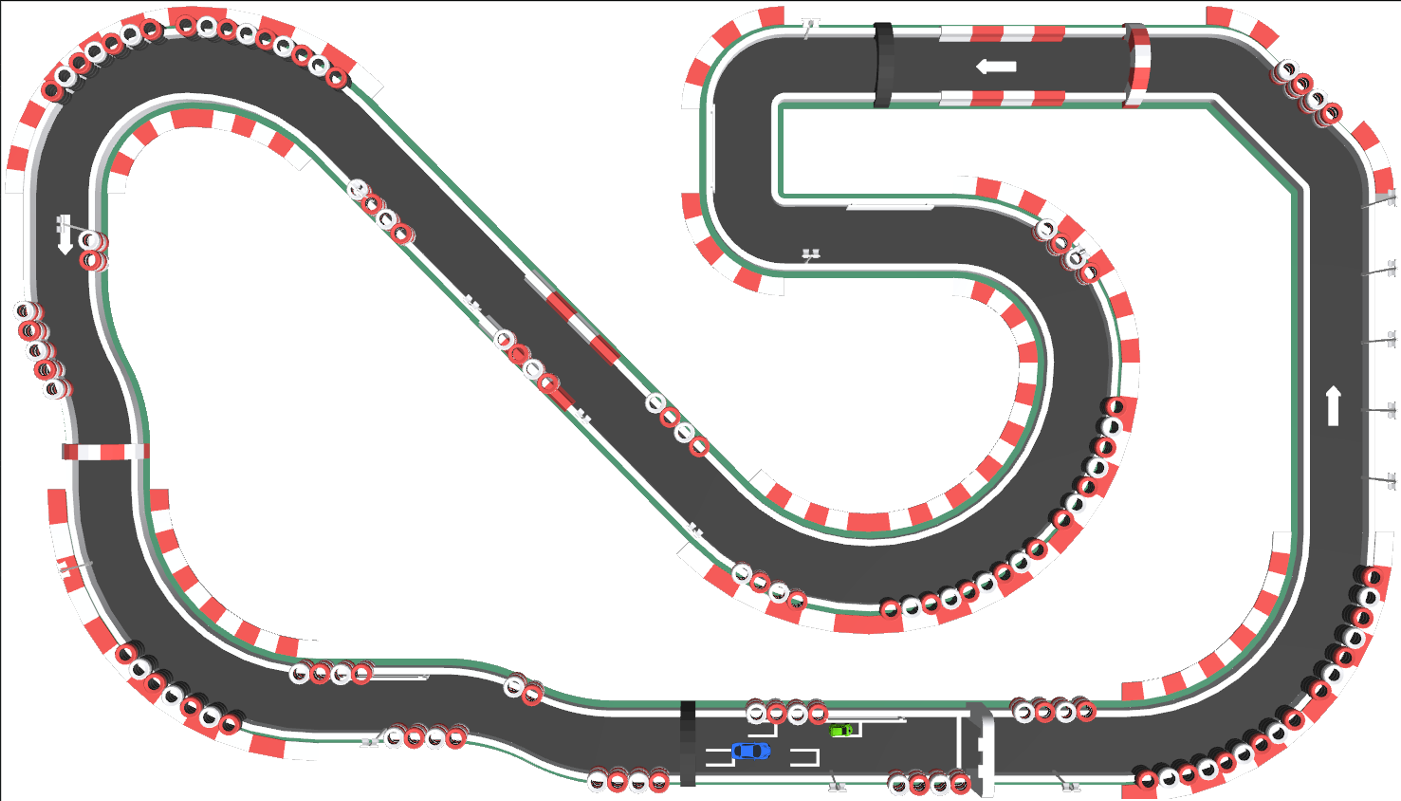
\includegraphics[scale=0.14]{images/overhead.png} }}%
    \qquad
    \subfloat[\centering ]{{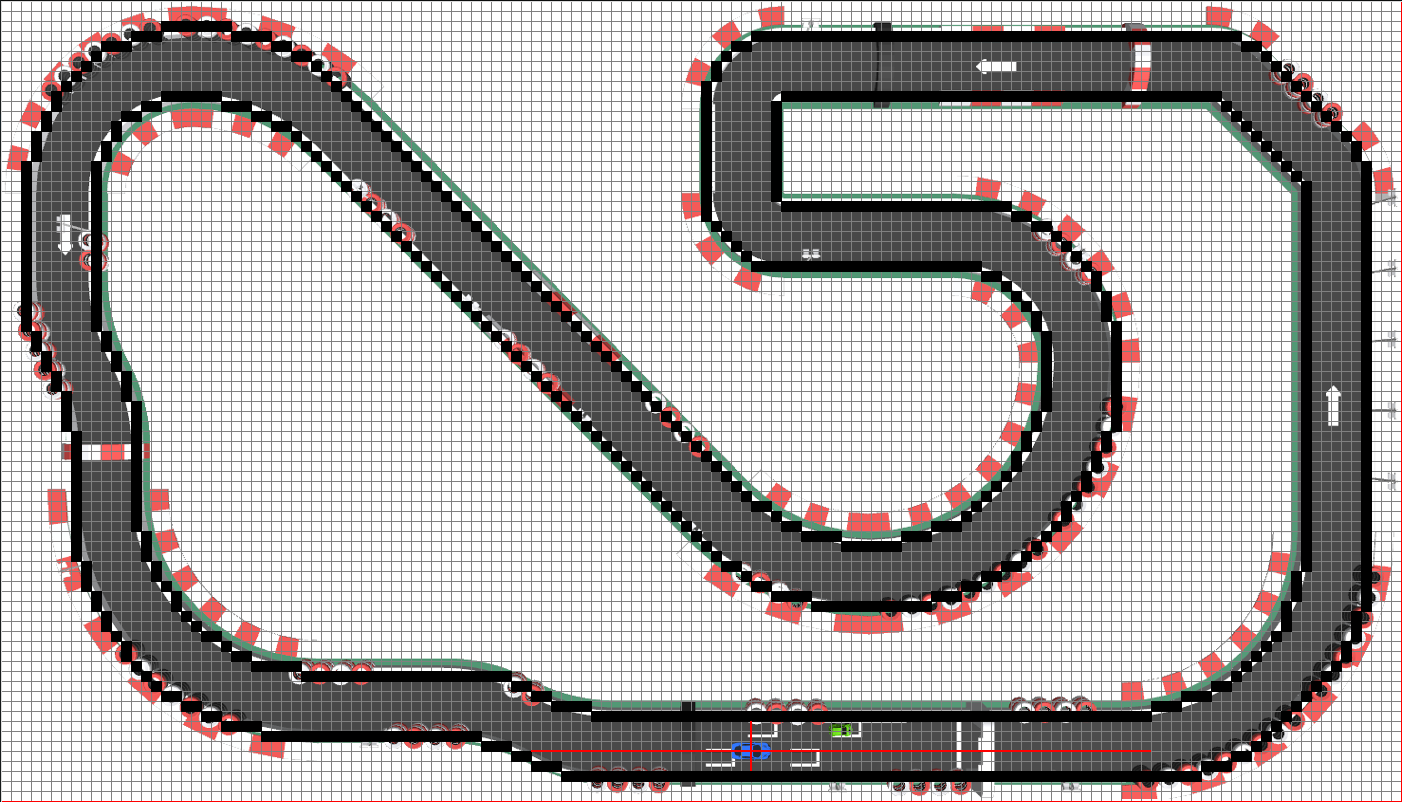
\includegraphics[scale=0.14]{images/grid.png} }}%
    \caption{Racetrack environment, with and without visualizing occupancy grid and sensor distances}%
    \label{fig:example}%
\end{figure}

\subsection*{Simulator}

Suppose for a moment that we want to set up an autonomous driving system to race a car around a racetrack, and we know the map of the racetrack ahead of time. In order to drive the car quickly around the track and avoid collisions, the system must know the current position of the car on the track (e.g., is the car on the racing line? is the car approaching the first turn?), as well as the direction in which the car is facing (e.g., is the car traveling straight down the road, or is it traveling toward a wall?), so that the system can generate the actions that are appropriate for the current state.

The problem of establishing the car's position and orientation in the map is called \textit{localization}. To simulate localization, we have set up a 2D racetrack and car inside of a simulator. The racetrack is located inside of a rectangular area 1400 units in width and 800 units in height. The car may move around the racetrack, but it can collide with the walls. The map is represented by an occupancy grid, where each cell is either 1 if a wall is present there, or 0 otherwise. The car has a throttle, brakes, and steering. The car also has range sensors that measure the direction in each of the 4 cardinal directions (North, South, East, West). The origin (0,0) of the coordinate system is in the top left corner, with x increasing to the right, and y increasing downward.

\subsection*{GUI}

When using the GUI, you can control various aspects of the simulator. You will need to use the GUI to visualize your results. Listed below are the available keyboard inputs. On Macs, you may need to press \texttt{command+<key>} (e.g., \texttt{command+o} to draw the occupancy grid and sensor readings).

\begin{tabbing}
    \texttt{↑ (ARROW UP)} \hspace{2em} \= Press throttle \\
    \texttt{↓ (ARROW DOWN)} \> Press brakes\\
    \texttt{← (ARROW LEFT)} \> Steer left\\
    \texttt{→ (ARROW RIGHT)} \> Steer right\\
    \texttt{o} \> Toggle drawing of occupancy grid and sensor readings\\
    \texttt{p} \> Toggle particle filtering\\
    \texttt{r} \> Toggle drawing of particles\\
    \texttt{k} \> Toggle Kalman filtering\\
    \texttt{d} \> Toggle GPS noise distribution\\
\end{tabbing}

\noindent
Of course, you have to implement the necessary code first for the particle filtering and Kalman filtering commands to work.\\

\noindent
Run \texttt{python3 gui.py -h} for info on how to specify parameters for particle filtering and Kalman filtering. Example usage:\\

\texttt{python3 gui.py --num\_particles 100 --max\_sensor\_range 100 --sensor\_noise\_std 2.0}\\

\subsection*{plots.py}

Run \texttt{plots.py} from the terminal to automatically generate plots for particle filtering and Kalman filtering using a pre-recorded drive around the track. Type \texttt{python3 plots.py -h} for info on how to specify parameters. Example usage for particle filtering (pf):\\

\noindent
\texttt{python3 plots.py -w pf --num\_particles 100 --max\_sensor\_range 100 --sensor\_noise\_std 2.0 --filename pf.png}\\\\

Example usage for Kalman filtering (kf):\\

\texttt{python3 plots.py -w kf --gps\_noise\_dist gaussian --gps\_noise\_var 4.0 --filename kf.png}\\

Plots will be stored inside the \texttt{plots} directory.

\subsection*{What you need to do}

\begin{enumerate}
    \item Complete all tasks listed below as Task 1.*, Task 2.*, Task 3.*. Some tasks will come in the form of multiple choice questions on Gradescope. \textbf{If so, just answer those questions. No extra responses are necessary.}
    \item Submit your answers to Gradescope by the deadline.
    \item Submit your code to Gradescope.
\end{enumerate}

\subsection*{Submission requirements}

\begin{itemize}
    \item While you are encouraged to collaborate, discuss and compare results with your classmates, your final code and responses submitted should be your own work.
    \item Keep your answers brief but reasonably thorough. The best response is one that is accurate and rigorous, while using as few words as possible.
    \item For coding tasks, write all your code in the sections bounded by
\end{itemize}

\begin{verbatim}
# BEGIN_YOUR_CODE ######################################################
\end{verbatim}
and
\begin{verbatim}
# END_YOUR_CODE ########################################################
\end{verbatim}

\subsection*{What to submit}

Answer the questions corresponding to each task on Gradescope. Assemble the following directory structure, compress \texttt{main\_directory} to .zip, and submit the .zip file to Gradescope.

\begin{tabbing}
    \texttt{main\_directory} \hspace{5em} \= Main directory \\
    \hspace{1em}\texttt{particle\_filter.py} \> Particle filtering code. \\
    \hspace{1em}\texttt{bayesian\_network.py} \> Bayesian network code.\\
    \hspace{1em}\texttt{kalman\_filter.py} \> If you attempted the extra credit Kalman filtering task.\\
    \hspace{1em}\texttt{plots.py} \> If you edited plots.py. Include any other plotting files as well.\\
    \hspace{1em}\texttt{README\_plots} \> If your plotting commands are different, describe how to use them.
    % \hspace{1em}\texttt{pf\_extra\_credit} \> Directory for the extra credit particle filtering task.\\
    % \hspace{2em} \texttt{particle\_filter.py} \> Your modified particle filtering code.\\
    % \hspace{2em} \texttt{...} \> Include \textbf{all} other files described below*\\
    % \hspace{2em} \texttt{README\_extra\_credit} \> If your commands are different, describe how to use them in detail.
\end{tabbing}

% \noindent
% \textbf{*If you did the extra credit task for particle filtering,} you must submit a separate directory containing a standalone implementation of the enhanced localization system. You may reuse or modify any files from the project repo. Running your code must involve simply switching to this directory and running the commands described in subsections \textbf{GUI} and \textbf{plots.py} above, but if you use different commands, include a README describing how to use them.

% \subsection*{Suggestions}

% You have 3 weeks to complete these tasks. Code for particle filtering should be less than 30 lines of code (approx), the coding portion for Bayesian networks is mostly counting, and Kalman filtering (extra credit) mostly involves setting the parameters of the Kalman filter from \texttt{filterpy}. I suggest you aim to finish particle filtering in the first week or early in the second week, and Bayesian networks in the second week. Continue to Kalman filtering (extra credit) if time permits.

%\subsection*{Grading}

\section{Particle Filtering}

In this section, you will create a particle filter to find the position and orientation of the car in the racetrack, given a known map of the racetrack and range sensor readings (distances to walls) from sensors on the car. You will not need to implement the entire algorithm from scratch---instead, we have provided some scaffolding in which you will write some important pieces of code.

\begin{figure}[h!]
    \centering
    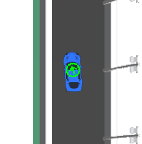
\includegraphics[scale=0.7]{images/pf_loclalized_crop.png}
    \caption{Estimated position and orientation after convergence of example particle filter.}
    \label{fig:pf_localized_crop}
\end{figure}

Your particle filter will initialize a set of particles uniformly randomly within the known bounds of the map. Each particle represents a possible location and orientation given the information seen so far; collectively, the set of particles represents a distribution of possible locations and orientations. As new information comes in, your particle filter will update the particles to more accurately reflect the true distribution. At each moment, your particle filter will use its distribution to compute a single estimation of position and orientation of the car. Your particle filter is expected to eventually converge to a distribution which accurately reflects the true distribution, and estimate a position and orientation which is approximately equal to the true position and orientation, as shown in Figure \ref{fig:pf_localized_crop}.\\

When running the particle filter (\texttt{p} key), the simulator (\texttt{simulator.py}) will construct a \texttt{ParticleFilter} object from \texttt{particle\_filter.py}, which initializes its particles throughout the map by calling \texttt{initialize\_particles}, a method you will implement. After updating the position and orientation of the car on each loop of the simulator, the loop will call \texttt{filtering\_and\_estimation} on its \texttt{ParticleFilter} object, to perform a single filtering step and compute a new estimate of position and orientation. This method invokes \texttt{filtering}, a method you will implement to perform the particle filtering algorithm given in the \href{https://github.com/aimacode/aima-pseudocode/blob/master/md/Particle-Filtering.md}{\textsc{Particle-Filtering} pseudocode} found in the AIMA textbook. In your implementation of \texttt{filtering}, you should call \texttt{transition\_sample} and \texttt{compute\_prenorm\_weight}, both of which you will also implement. This amounts to completing four methods listed below in Task 1.1:\\

\noindent
\textbf{Task 1.1} Complete the implementation of the particle filter in \texttt{particle\_filter.py} to track the location and orientation of the car in the map. Methods to edit:\\

\indent \texttt{initialize\_particles}\\
\indent Initializes the particles uniformly randomly within the bounds of the rectangular region.\\

\indent \texttt{transition\_sample}\\
\indent Samples a next pose for a given particle according to the car's transition model.\\

\indent \texttt{compute\_prenorm\_weight}\\
\indent Computes the pre-normalization weight of a particle given evidence, such that normalizing the\\
\indent pre-normalization weights for all particles gives your $P($evidence$\mid$particle pose$)$ for each particle.\\

\indent \texttt{filtering}\\
\indent Performs one step of particle filtering according to particle-filtering pseudocode in AIMA.\\
\indent This should closely resemble their pseudocode.\\

\noindent The file \texttt{particle\_filter.py} is heavily commented so you can know what exactly these methods need to do. There are some hints inside these methods, as well. The comments should be helpful, so read through them. You can complete this task in just 20 lines of code.\\

\noindent
Hint: when tuning your parameters, make sure you tune the std of the Gaussian kernel, since this will define how much you penalize sensor readings that are very dissimilar to the car's readings (which is what happens often when the particles are clustered somewhere far away from the car). A sensible thing to do in this case is to give such particles 0 weight. \texttt{weighted\_sample\_w\_replacement} will re-initialize the particles automatically when the weights of the particles are all 0, so you should set your Gaussian kernel std so that the Gaussian function is very close to 0 for very high inputs (high distance in vector space), and zero out any values less than some small threshold of your choosing (e.g., 0.001). The default value of \texttt{std=500} is arbitrary. Try much lower values.\\

\noindent
\textbf{Task 1.2} Fix maximum sensor range to 400 and standard deviation of sensor noise to 2.0. Estimate the lowest particle count that reliably localizes the car by manually tuning this parameter (you probably will want to use \texttt{plots.py} for visualization instead of the GUI). Assume that ``reliably'' here means that 9 out of 10 times, it will localize the car before it exits the first turn, and follow the car around the track all the way to the end. You may set any other parameter to an appropriate value. Plot the estimated path and error using \texttt{plots.py}, and submit the plots along with the particle count you used.\\

\noindent
\textbf{Task 1.3} Characterize the dependence of accuracy and efficiency on sensor noise, number of particles, and max sensor range. Efficiency is in terms of time complexity. Support your assertions using quantitative or anecdotal evidence (the more rigorous, the better). Relationships to characterize: (accuracy vs noise), (accuracy vs number), (accuracy vs range), (efficiency vs noise), (efficiency vs number), (efficiency vs range).\\

\noindent
\textbf{Task 1.4} What probabilistic assumptions are we making about the state transition model? How well do these assumptions match the true state transition model? In what way and to what extent is performance affected by making these assumptions?\\

\noindent
\textbf{Task 1.5} Describe some cases in which the particle filter fails to localize the car in this map, and explain why this happens.\\

\begin{figure}[b!]
    \centering
    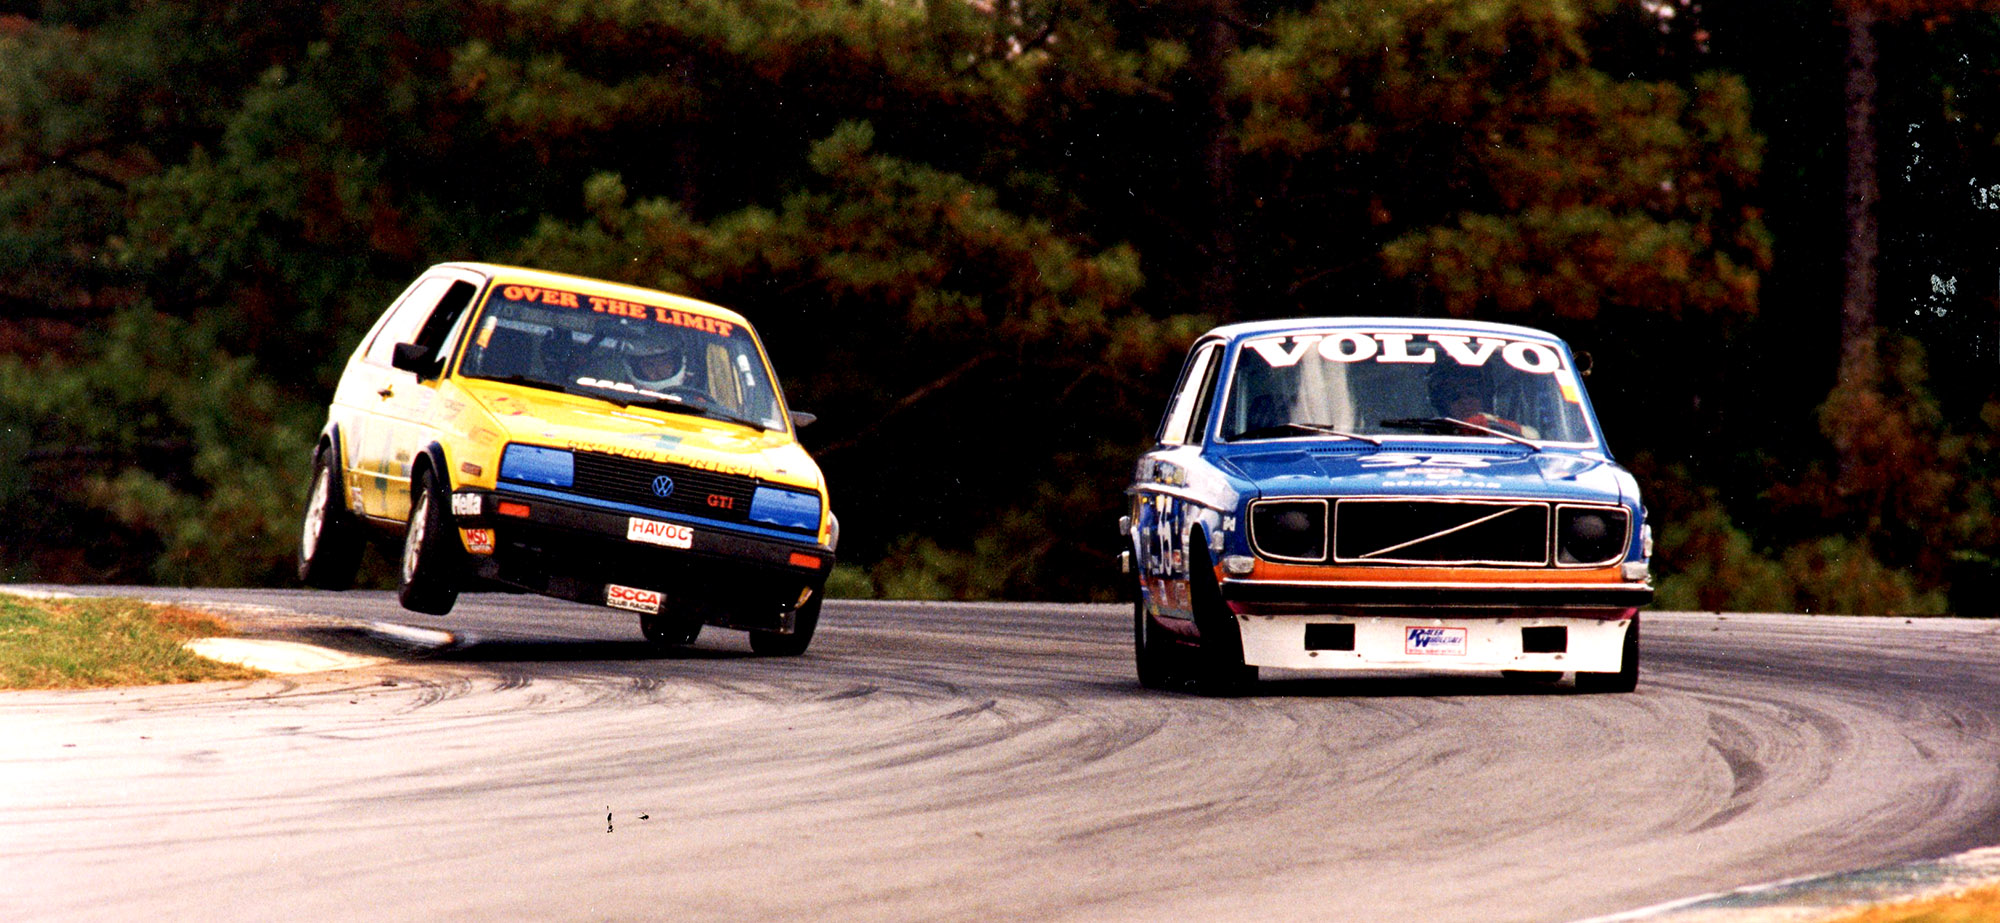
\includegraphics[scale=0.4]{images/overtake.jpg}
    \caption{Two cars racing through a turn.}
    \label{fig:overtake}
\end{figure}

\section{Bayesian Networks}

Suppose we are racing an opponent car up the diagonal road in the middle of our racetrack, approaching the second-to-last turn in the race before the finish line. We are behind our opponent, but we are moving faster toward the turn, and we are going to attempt to overtake them through this turn to win the race. In order to win the race, we must overtake the opponent car (eventually), ideally without colliding with the tires, though a small collision does not rule out the possibility of victory. Our ability to overtake the other car in this turn depends, in part, on how much faster we are traveling than the other car, and how close we are to the turn (e.g., an early overtake attempt at much higher speed is more likely to succeed than a late overtake attempt when we're not moving much faster than the opponent). Similarly, our ability to avoid collision depends on how much faster we are traveling and how close we are to the turn (e.g., if we're traveling too fast and attempting the overtake too late, then we might miss the apex and crash hard into the tires).\\

\noindent
\textbf{Task 2.1} Let $MuchFaster\in \{T,F\}$ represent whether we are moving much faster than the opponent (as opposed to just a little faster), $Early\in \{T,F\}$ represent whether the attempt is early, $Overtake\in \{T,F\}$ represent whether we overtook the opponent \textbf{in the second-to-last turn}, $Crash\in \{T,F\}$ represent whether we crashed, and $Win\in \{T,F\}$ represent whether we win the race. Draw the structure of the Bayesian network that represents the conditional dependencies described in this situation (and no other dependencies), using only the given variables. Assume $MuchFaster$ and $Early$ are independent.\\

\noindent
\textbf{Task 2.2} Suppose we have recorded 1000 different overtake attempts on this racetrack, and we want to model the joint probability distribution $P(MuchFaster,Early,Overtake,Crash,Win)$. For each instance, we have recorded the values for $MuchFaster,Early,Overtake,Crash,$ and $Win$ as $True$ or $False$, and stored the data points inside of a dataset. Instantiate your Bayesian network from Task 2.1 as a \href{https://github.com/aimacode/aima-python/blob/master/probability.py#L164}{\texttt{BayesNet} from the AIMA code repository}, complete with conditional probability tables for each node. Write your code inside the method \texttt{generate\_bayesnet} in \texttt{bayesian\_network.py}.\\

\noindent
Hint: To estimate probabilities, use frequencies of occurrences in the dataset (e.g., estimate $P(Alarm=T,Burglary=F)$ as $\frac{\textnormal{number of data points with } Alarm=T,Burgulary=F}{\textnormal{total number of data points}})$.\\

\begin{figure}[b!]
    \centering
    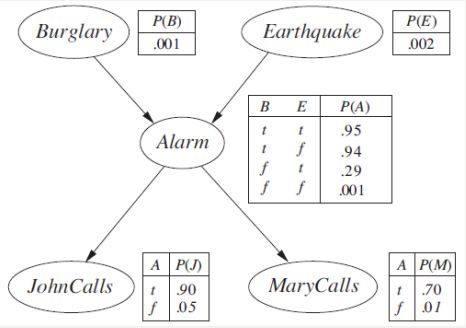
\includegraphics[scale=0.47]{images/bayesnet.png}
    \caption{Bayesian network from AIMA.}
    \label{fig:burglary}
\end{figure}

\noindent
Hint: If you were to construct a BayesNet for the network in Figure \ref{fig:burglary}, you would write the following code:
\begin{verbatim}
T, F = True, False

burglary = BayesNet([
    ('Burglary', '', 0.001),
    ('Earthquake', '', 0.002),
    ('Alarm', 'Burglary Earthquake',
     {(T, T): 0.95, (T, F): 0.94, (F, T): 0.29, (F, F): 0.001}),
    ('JohnCalls', 'Alarm', {T: 0.90, F: 0.05}),
    ('MaryCalls', 'Alarm', {T: 0.70, F: 0.01})
])
\end{verbatim}
The BayesNet constructor takes a list of node specifications (variable,parents,CPT), where variable is the name of the variable, parents is a string listing the names of parent nodes joined by spaces (empty string if there are no parents), and CPT is the conditional probability table represented as a dictionary, or just probability if there are no parents. The list must be ordered so that parent nodes come before child nodes.\\

\noindent
\textbf{Task 2.3} Using the network you generated, determine the overtaking condition (values for $MuchFaster$ and $Early$) that yields the highest probability of winning the race without crashing. Write your code inside \texttt{find\_best\_overtake\_condition} in \texttt{bayesian\_network.py}. Your code should display the correct answer when you run \texttt{python3 bayesian\_network.py} from the command line. Write the mathematical formula that represents this optimal overtaking condition in terms of conditional probabilities found in the Bayesian network.\\

\noindent
Hint: Use any one of the following methods from \texttt{probability.py} to compute a conditional probability using your BayesNet: \texttt{enumeration\_ask, elimination\_ask, rejection\_sampling, likelihood\_weighting, gibbs\_ask}. We've already imported them for you. Example usage: to use variable elimination to compute the distribution $P(Burglary|JohnCalls=T,MaryCalls=T)$ on the burglary network, you would call \texttt{elimination\_ask('Burglary', dict(JohnCalls=True, MaryCalls=True), burglary)}.

\section{Kalman Filtering (Extra Credit)}

\noindent
\textbf{Task 3.1} Implement a Kalman filter to track the location and velocity of the car in the map given noisy GPS measurements of the car's position. Write your code in \texttt{kalman\_filter.py}. You may use a Kalman filter from FilterPy. You should only need to set the parameters of the \texttt{KalmanFilter} object in the constructor, and write a couple of lines to perform prediction and updating (see \href{https://filterpy.readthedocs.io/en/latest/kalman/KalmanFilter.html}{here} for a list of parameters and for an example prediction/update).\\

\noindent
\textbf{Task 3.2} Explain how you set your parameters.\\

\noindent
\textbf{Task 3.3} Run the standard plot code in \texttt{plots.py} to generate plots, and submit them. Characterize the dependence of accuracy on measurement noise and measurement distribution (generate plots for Gaussian and uniform noise distributions, with different variance and width). Support your assertions using quantitative and/or anecdotal evidence (the more rigorous, the better).\\

\noindent
\textbf{Task 3.4} What assumptions does the Kalman filter make about the GPS measurements? How well do these assumptions match the process that generates the data? In what way and to what extent is performance affected by these making these assumptions?\\

\end{document}